\chapter{競合するサービスとの比較}\label{ux4ed6ux306eux30bdux30d5ux30c8ux3068ux306eux6bd4ux8f03}
現在,インターネット上にはプログラミング言語の学習を目的としたサービスが多く存在する.
その中でも人気のサービスは,ドットラーニング\cite{ドットラーニング},paizaラーニング\cite{paiza},progate,codecademyがあげられる.
それらのサービスと本研究で開発したアプリケーションとの比較を以下に示す.
\begin{table}[H]
\centering
\begin{center}
\caption{競合サービスの比較.\label{service_compare}}
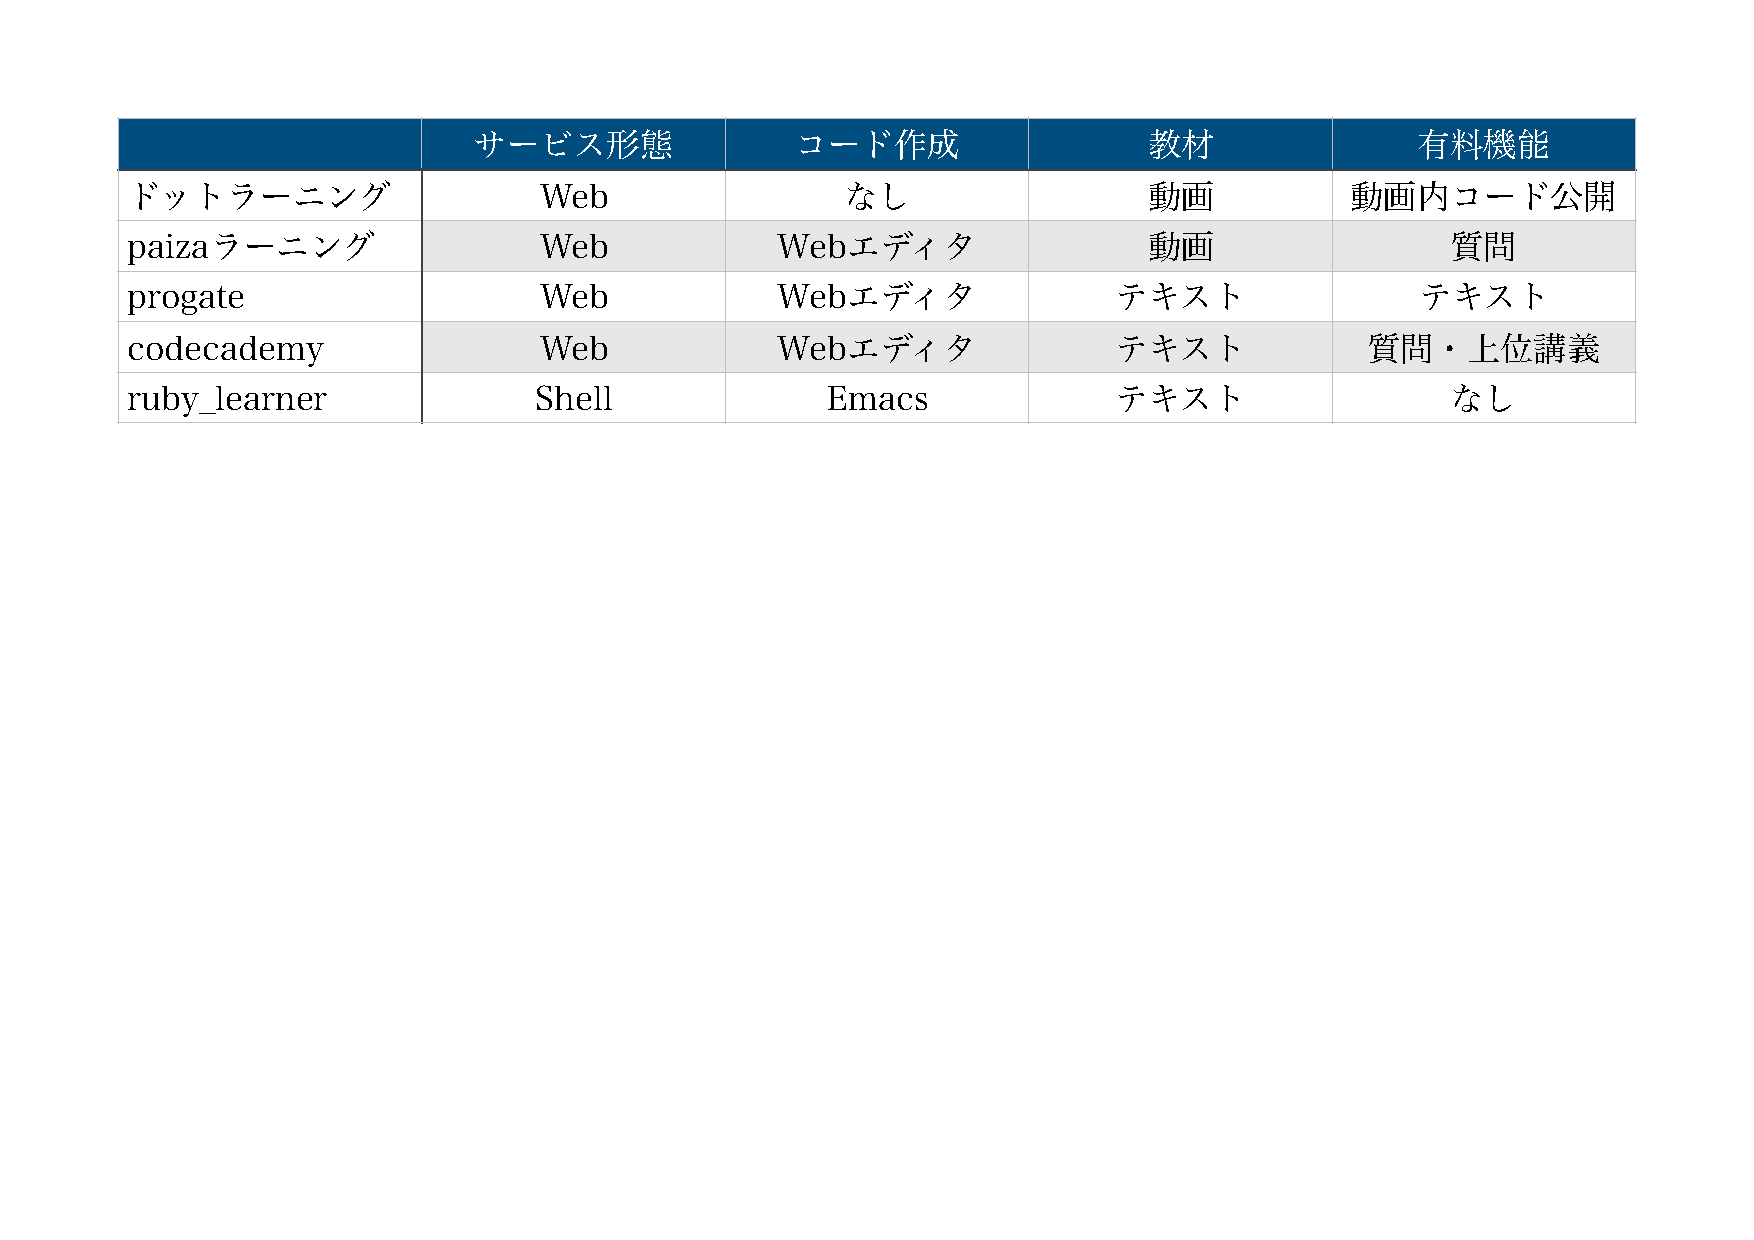
\includegraphics[width=150mm]{../../picture/service_compare.pdf}
\end{center}
\label{fig:}
\end{table}

\section{考察}\label{ux8003ux5bdf}
ruby\_learnerを除く一般的なサービスはGUIで操作するWebサービスである.しかし,実際の開発環境はWebではなくshellで行う場合が多いと考えられる.また,サービス内で使用するコード記入に用いられるエディタはruby\_learner以外はサービス外で行う開発には用いることはできない.上記の2点からも分かるように,実際の開発体験に近い環境での学習ではruby\_learnerが優れており,サービス外での学習へのサポートも兼ね備えていることがわかる.また有料機能がない点で,使用者にストレスレスな学習を提供できると考えられる.本研究で作成したアプリケーションのソースコードはGithub上に掲載しており,OSS開発を行えるようにしている.これにより今後の機能追加が可能となっているので,さらに学習に必要とされる機能に関しては順次追加することもできる.
